\section{The Wollok Language}
\label{sec:wollokLanguage}

% Free form, variable number of sections, technical details.
% But in general do not mix solution and discussions/possible variation let that for discussion

Wollok is a brand new languages built to specifically give support to our pedagogical approach~\cite{lombardi_instances_2007,lombardi_carlos_alumnos_2008}. 
Wollok provides an extremely simple programming model which allows the students to create programs containing objects, messages and polymorphism without the need for more abstract concepts such as classes, inheritance or type annotations.
Later in the course, Wollok allows the incremental introduction of more abstract concepts,
providing a smooth transition into a full-fledged OO programming model.

The example in figure \ref{fig:helloWorld/wollok} shows an example first program in a Wollok-based OO introductory course.
Syntax has been reduced to a minimum and the basic constructs of the language match exactly the concepts we want to transmit, \eg \code{var} is used to define variables and \code{method} is used to define methods.
The \code{accumulator} object is defined as a stand-alone (\ie it has no visible class), automatically instantiated and \emph{well-known} (\ie globally accesible) object (WKO).

\vspace{-3mm}
\begin{figure}[ht]
 \centering
 \begin{lstlisting}[language=Wollok]
	object accumulator {
		var total = 0
		var evens = 0
		
		method getCurrentTotal() { return total }
		method add(amount) { 
			total += amount 
			if (amount % 2 == 0) { evens += 1 }
		}
		method evenCount() { return evens }
	}\end{lstlisting}
\vspace{-3mm}
\caption{\small Sample initial Wollok object definition.}
\label{fig:helloWorld/wollok}
\end{figure}

We put special emphasis in avoiding input and output (I/O). 
Normally, writing to standard output as it is shown in Fig. \ref{fig:helloWorld} will be considered a problem in industrial software construction.
Therefore, teaching the students to try out their programs in this way is introducing a bad practice that will have to be \emph{unlearned} later.
On the other hand, we need some kind of user interaction to be able to see the behaviour of our programs. However, proper handling of user interaction is way beyond the scope of an initial OO course.

The first tool we introduce to try out a program without requiring I/O is a \emph {read-eval-print-loop}~(REPL). Running a program in the REPL brings all defined objects to life and allows the user to interact with them sending messages, as shown in Fig.~\ref{fig:repl}. 
The REPL handles all I/O and the student is only required to write the desired messages to a \emph{domain object}.

\begin{figure}[ht]
 \centering
 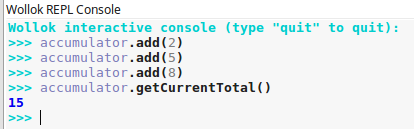
\includegraphics[scale=0.6]{images/accumulator-repl.png}
 \caption{\small Sample usage of the accumulator object in the REPL}
 \label{fig:repl}
\end{figure}


%This is also consistent with some modern industrial OO languages that allow to define both classes or standalone objects, such as Scala \cite{Oder04a}.

%To build this first program students are not required to know about typing, scoping or packaging.
%The only required construct is the \code{program} and the only command is a message send.
%Both the receiver and the parameters are built-in objects which will be handled in the same way as user-defined objects.
%The concepts required to understand this program are no more than program, object, message and argument passing.

Shortly after in the course, we introduce unit testing which slowly replaces the REPL as the main form of interacting with objects. Figure \ref{fig:test} shows a sample test for the previous program. 

\begin{figure}[ht]
 \centering
 \begin{lstlisting}[language=Wollok]
 	import accumulator.*

	test "adding 2+5+8 should give 15" {
		accumulator.add(2)
		accumulator.add(5)
		accumulator.add(8)
		assert.equals(15, accumulator.getCurrentTotal())		
	}
   
	test "accumulator starts with 0" {
		assert.equals(0, accumulator.getCurrentTotal())
	}\end{lstlisting}
\vspace{-3mm}
\caption{\small Sample test Wollok program.}
\vspace{-5mm}
\label{fig:test}
\end{figure}

Again, Wollok is fine-tuned for our pedagogical objectives.
In particular, the test runner guarantees that there is no interaction between tests: the messages sent to the accumulator in the first test will not affect the state of the accumulator in the second test\np{sería lindo tener una cita a alguna regla de unit testing que proponga esto}.
Furthermore, tests have to be written in a separate file.
However, this decision introduces a problem: the objects (and later on, classes) defined in a different file must be accesible from the test file. With this purpose, Wollok includes a simple form of the \texttt{\textbf{import}} directive, which refers to a object/class definition file in the same folder than the test file. In this way, some basic knowledge of modularization is subtly introduced early in the course\footnote{The assimilation of the \texttt{import} directive, as early as in the second week, was not problematic in our experience using Wollok for first-year programming courses.}.

%Tests have to be written in a separate file; the directive \texttt{
%\textbf{import} accumulator.*} at the beginning of the example indicates that all the objects (and later on, classes) defined in the file called \texttt{accumulator.wlk} are available to be used in the test. In this way, some basic knowledge of modularization is subtly introduced at the very beginning of the course\footnote{\carlostext{The assimilation of the \texttt{import} directive at the second week, was not problematic in our experience using Wollok for first-year programming courses.}}. 
%Furthermore, }
%For example, tests have to be written in a separate file, which introduces the student into some basic knowledge of modularization.
%Also, 
%the test runner guarantees that there is no interaction between tests: the messages sent to the accumulator in the first test will not affect the state of the accumulator in the second test\np{sería lindo tener una cita a alguna regla de unit testing que proponga esto}.

\medskip
% Misceláneos
% Profundizar y pulir el highlighting the conceptos primarios y la estratificacion de conceptos
Another simple feature that is very helpful in the initial steps of the course is the presence of literals for lists (\eg \code{[1,2,3]}) and sets (\eg \code{\#\{1,2,3\}}).
This allows us to use collections and, therefore, increase the complexity of examples that we can build before introducing classes.
We even briefly introduce \emph{closures} at the initial stage of the course.
For example, our \code{accumulator} object can be implemented as shown in Fig. \ref{fig:accumulator/list}.
%Also \emph{Collection literals} reduce boilerplate on object creation, 
%since we think that the excess of bureaucracy to create an object helps to build up 
%the belief that using objects or collections is far more complicated than using numbers or strings, which in turns leads to \emph{primitive obsession} \cite{fowler_refactoring:_1999}.

\vspace{-3mm}
\begin{figure}[ht]
 \centering
 \begin{lstlisting}[language=Wollok]
	object listBasedAccumulator {
		var history = []
		
		method getCurrentTotal() {
			return history.sum()
		}
		method add(amount) { history.add(amount) }
		method evenCount() {
		  return history.count({n => n % 2 == 0})
		}
	}\end{lstlisting}
\vspace{-3mm}
 \caption{\small Another accumulator implementation, using a list.}
\vspace{-3mm}
 \label{fig:accumulator/list}
\end{figure}

\medskip
Next in the course, we introduce classes.
Once more, Wollok helps us in the transition: any pre-existent stand-alone object can be converted into a class by just changing the keyword \code{object} for \code{class}\footnote{As a matter of fact, we will also change the name, as our code convention mandates lowercase names for objects and uppercase names for classes}, as shown in Fig. \ref{fig:accumulator/classes}.

\begin{figure}[ht]
 \centering
 \begin{lstlisting}[language=Wollok]
	class ListBasedAccumulator {
		var history = []
		
		method getCurrentTotal() { 
			return history.sum() 
		}
		method add(amount) { history.add(amount) }
		method evenCount() { 
		  return history.count({n => n % 2 == 0})
		}
	}\end{lstlisting}
\vspace{-3mm}
\caption{\small A third accumulator implementation, class based.}
\label{fig:accumulator/classes}
\end{figure}

Figure \ref{fig:polymorphism} shows how the three previous definitions of accumulator can be used polymorphically. 
\cl{la siguiente frase, incluyendo el footnote, es reemplazada por el texto que propongo agregar al introducir colecciones.}
Also, it shows the usage of more advanced list messages and closures\footnote{In our approach, we introduce polymorphism and closures \emph{before} classes. For reasons of space we skipped those intermediate examples here.}.
A special mention has to be made about the fact that stand-alone objects are used in the same program and even they are polymorphic with class-based objects.

\begin{figure}[ht]
\vspace{-3mm}
 \centering
 \begin{lstlisting}[language=Wollok]
 	import accumulator.*

	test "adding 2+5+8 should give 15" {
		const accumulators = [ 
			accumulator, 
			listBasedAccumulator,
			new ListBasedAccumulator()
		]

		accumulators.forEach { accum =>
			accum.add(2)
			accum.add(5)
			accum.add(8)
			assert.equals(15, accum.getCurrentTotal())	
		}
	}\end{lstlisting}
\vspace{-3mm}
\caption{\small Simple polymorphism example.}
\label{fig:polymorphism}
\end{figure}

% Effect
Finally, Wollok includes features that allow for discussing about \emph{controlling side effects} in an early stage of programming courses, making programmers aware of the potential side effects of each portion of code.
The most basic of these features is the ability to 
differentiate variables from constants (defined using \code{var} and \code{const} resp.).
Moreover, methods not including a \texttt{return} expression are considered as \emph{void}, \ie\ they do not yield a value and no operation can be applied to them. Furthermore, the REPL does not show any text as result of the evaluation of void methods, as can be seen in Fig.~\ref{fig:repl}.
